\section{Results \& Discussion}
\label{sec:result}
\ref{fig:sim_result} indicates the result of gossip-based aggregation averaging simulation as illustrated in section~\ref{sec:simulation}. 
\begin{figure}[h!]
	\centering
    \begin{subfigure}[t]{0.47\textwidth}
    \vspace{0pt}
    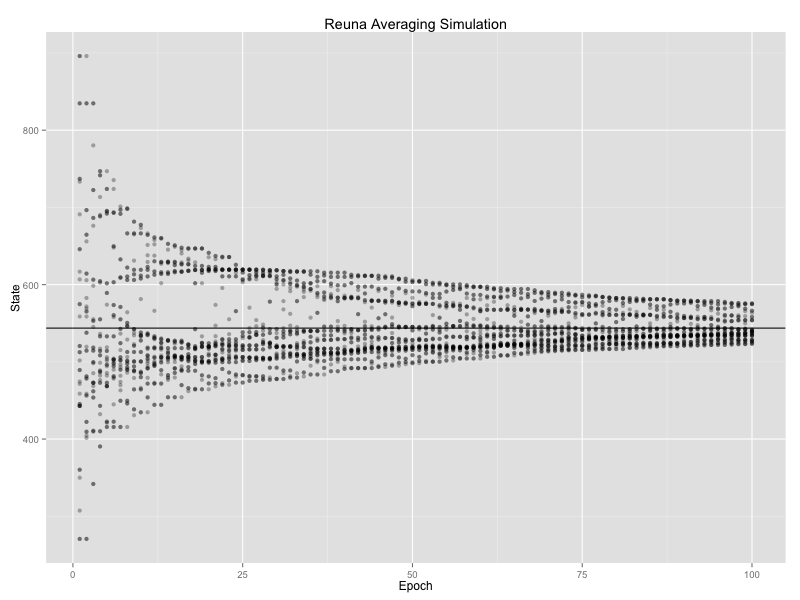
\includegraphics[width=\linewidth]{figures/Simulation_averaging/ReunaAvgSim.png}
    \caption{Reuna Averaging Simulation}
    \end{subfigure}
    %\vspace{5ex}
    \begin{subfigure}[t]{0.47\textwidth}
    \vspace{0pt}
    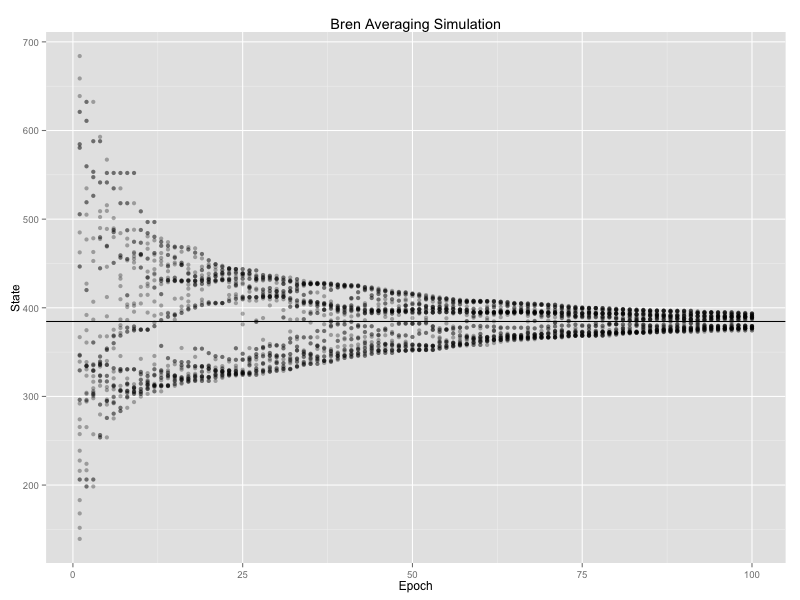
\includegraphics[width=\linewidth]{figures/Simulation_averaging/BrenAvgSim.png}
    \caption{Bren Averaging Simulation}
    \end{subfigure}
    \vspace{5ex}
    \begin{subfigure}[t]{0.47\textwidth}
    \vspace{0pt}
    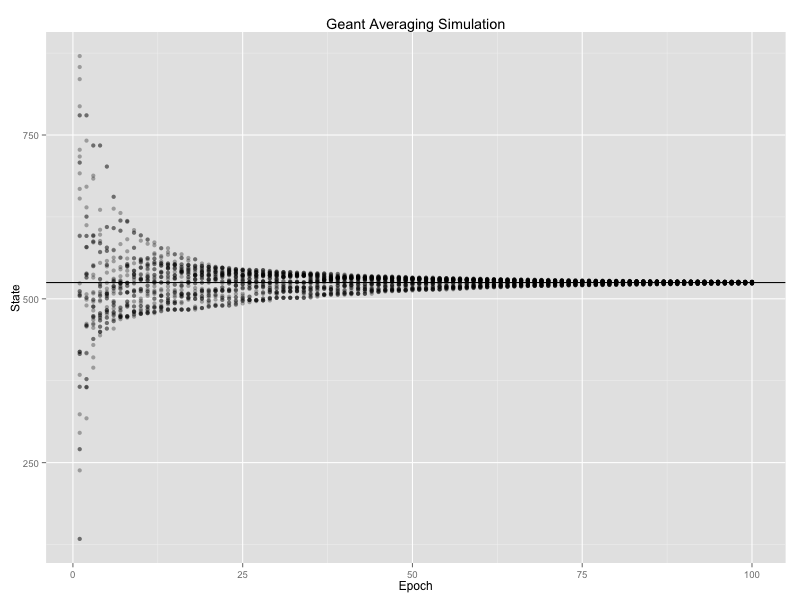
\includegraphics[width=\linewidth]{figures/Simulation_averaging/GeantAvgSim.png}
    \caption{Geant Averaging experiment}
    \end{subfigure}
    %\vspace{5ex}
    \begin{subfigure}[t]{0.47\textwidth}
    \vspace{0pt}
    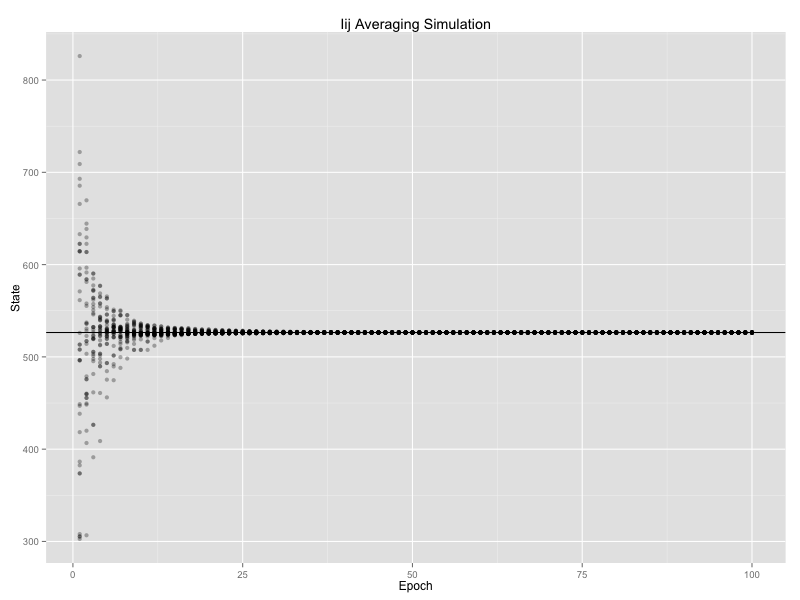
\includegraphics[width=\linewidth]{figures/Simulation_averaging/IijAvgSim.png}
    \caption{Iij averaging experiment}
    \end{subfigure}
    \caption{State changes of all nodes per epoch}
    \label{fig:sim_result}

\end{figure}
%TODO: define convergence criteria and derive the convergence speed.

\begin{figure}[h!]
	\centering
    \begin{subfigure}[t]{0.47\textwidth}
    \vspace{0pt}
    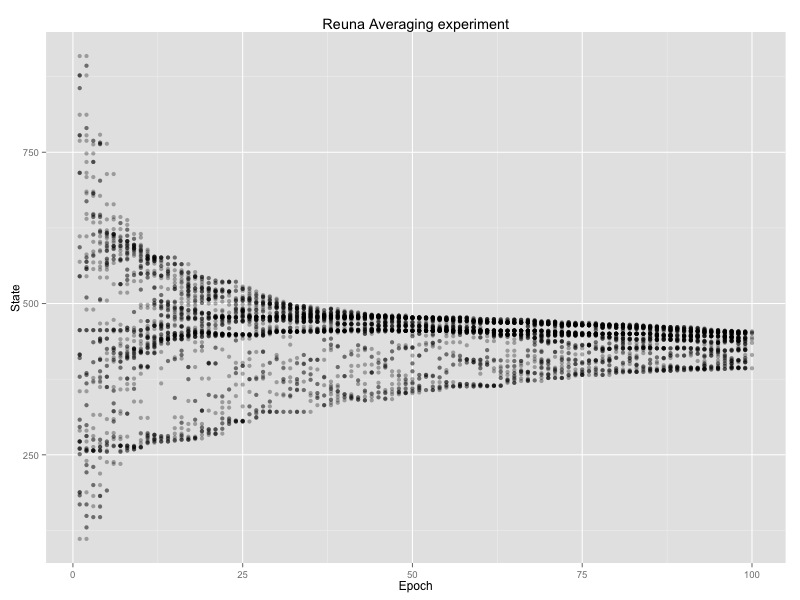
\includegraphics[width=\linewidth]{figures/Reuna.png}
    \caption{Reuna Averaging experiment}
    \end{subfigure}
    %\vspace{5ex}
    \begin{subfigure}[t]{0.47\textwidth}
    \vspace{0pt}
    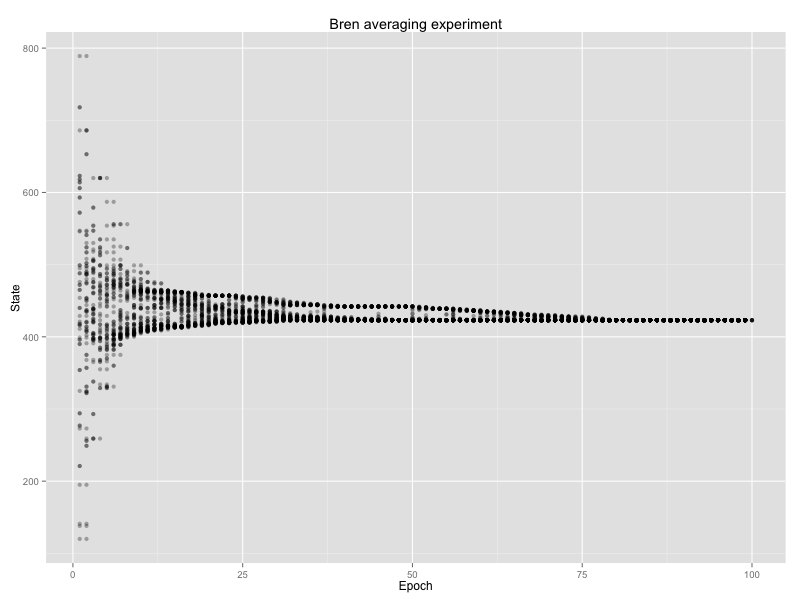
\includegraphics[width=\linewidth]{figures/Bren.png}
    \caption{Bren Averaging experiment}
    \end{subfigure}
    \vspace{5ex}
    \begin{subfigure}[t]{0.47\textwidth}
    \vspace{0pt}
    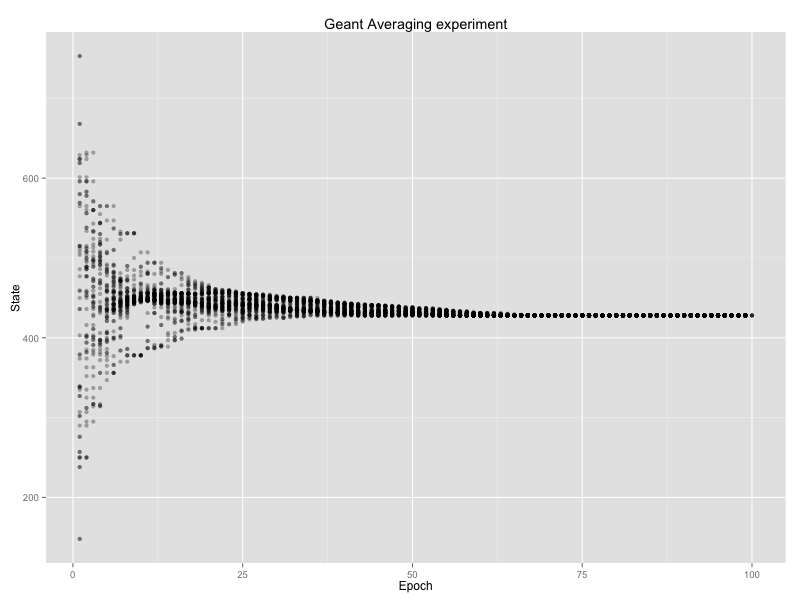
\includegraphics[width=\linewidth]{figures/Geant.png}
    \caption{Geant Averaging experiment}
    \end{subfigure}
    %\vspace{5ex}
    \begin{subfigure}[t]{0.47\textwidth}
    \vspace{0pt}
    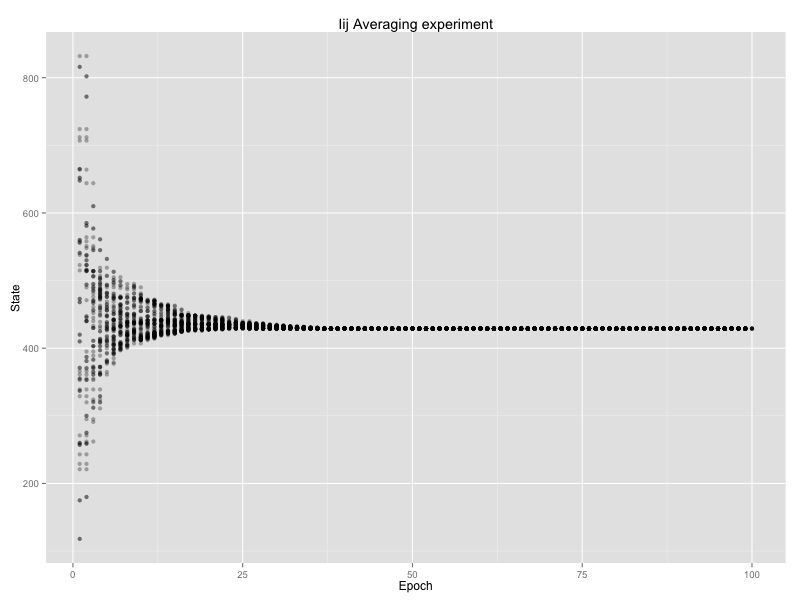
\includegraphics[width=\linewidth]{figures/Iij.png}
    \caption{Iij averaging experiment}
    \end{subfigure}
    \caption{State changes of all nodes per epoch}
    \label{fig:result}

\end{figure}
% aggregation of a random value from 0 to 1000
The results of our experiments are visualized in figure \ref{fig:result}. The X-axis are the epoch (time intervals) and the Y-axis is the state value. The gossip-based aggregation was run over 100 epochs. Every node started with a value chosen randomly between 0 and 1000. Due to the random nature of the algorithm and the difference in degree of connectivity among nodes a node can have between 1 and N state changes per epoch. (Where N is the amount of nodes in the network.) Overall nodes the number of state changes is 2*N per epoch. (Every node initiates one exchange per epoch which entails two state changes.) All of these changes are depicted.

The graphs are sorted according to number of links per nodes from left to right and top to bottom. Inside 100 epochs all four experiments are in the trend of converging and if we set convergence criteria as 5\% of mean value, Bren, Geant and Iij converge inside their run of experiments, accordingly at the 75th, 60th and the 40th epoch. Reuna does not converge during the 100 epochs of our experiment.

Thus, the order of convergence speed can be derived as Iij, Geant, Bren, Reuna, from the fastest to slowest, which supports our hypothesis.

\begin{figure}[h!]
    \begin{center}
    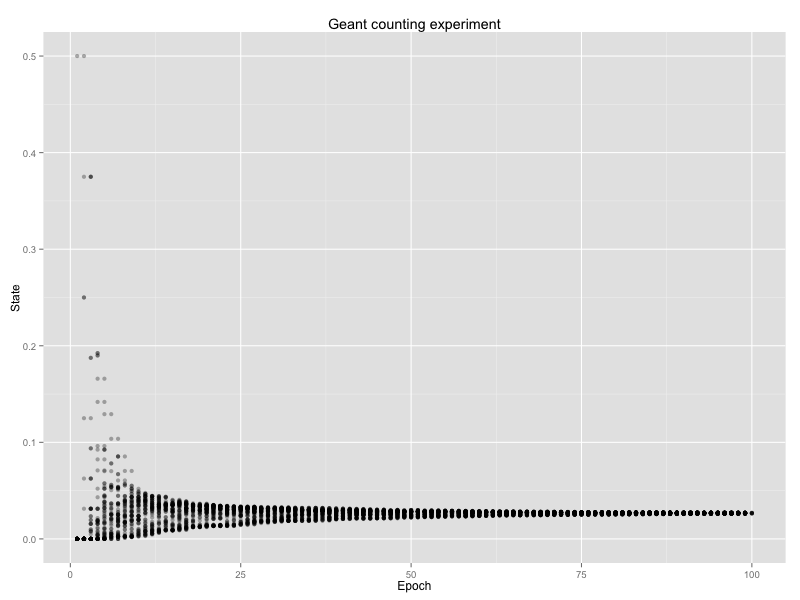
\includegraphics[scale=0.4]{figures/geant_counting_exp.png}
    \end{center}
    \caption{Geant counting}
    \label{fig:geant}
\end{figure}
\label{sec:results}
